\documentclass[10pt]{article}

\usepackage[utf8]{inputenc}

\usepackage{graphicx} % for figures
\usepackage{ccaption} % captions on different pages

%% BASED ON TEMPLATE GIVEN FOR PLOS

% amsmath package, useful for mathematical formulas
\usepackage{amsmath}
% amssymb package, useful for mathematical symbols
\usepackage{amssymb}

% cite package, to clean up citations in the main text. Do not remove.
\usepackage{cite}

\usepackage{hyperref}

% line numbers
\usepackage{lineno}

% ligatures disabled
\usepackage{microtype}
\DisableLigatures[f]{encoding = *, family = * }

% rotating package for sideways tables
%\usepackage{rotating}

% If you wish to include algorithms, please use one of the packages below. Also, please see the algorithm section of our LaTeX guidelines (http://www.plosone.org/static/latexGuidelines) for important information about required formatting.
%\usepackage{algorithmic}
%\usepackage{algorithmicx}

% Use doublespacing - comment out for single spacing
%\usepackage{setspace} 
%\doublespacing


% Text layout
\topmargin 0.0cm
\oddsidemargin 0.5cm
\evensidemargin 0.5cm
\textwidth 16cm 
\textheight 21cm

% Bold the 'Figure #' in the caption and separate it with a period
% Captions will be left justified
\usepackage[labelfont=bf,labelsep=period,justification=raggedright]{caption}

% Use the PLoS provided BiBTeX style
%\bibliographystyle{plos2009} % NOW in drosprpaper.tex

% Remove brackets from numbering in List of References
\makeatletter
\renewcommand{\@biblabel}[1]{\quad#1.}
\makeatother


% Leave date blank
\date{}

\pagestyle{myheadings}

%% Include all macros below. Please limit the use of macros.

%% END MACROS SECTION

%%% MY STUFF %%%

% my packages

\usepackage{gensymb}
\usepackage{setspace} % for 1.5 spacing
\usepackage{verbatim} % multiline comments
\usepackage{acronym}

\usepackage{rotating} % sidewaysfigure

\acrodef{RF}{receptive field}
\acrodef{RIDF}{rotational image difference function}
\acrodef{rms}[r.m.s.]{root mean square}
\acrodef{ANN}{artificial neural network}

%\usepackage{todonotes}
%\usepackage{soul}
%%\newcommand{\hltodo}[2]{\texthl{#1}\todo{#2}}
%\newcommand{\hltodo}{}
%\usepackage{pdfcomment}

% header stuff
\usepackage{fancyhdr}
\setlength{\headheight}{15.2pt}
\pagestyle{fancy}

\newcommand{\Matlab}{MATLAB}

%\newcommand{\thesiscontcaption}[1]{\caption[#1]{#1 (Continued on next page.)}}

\begin{document}

%\newcommand{\draft}{D8} %% NOW IN drosprpaper.tex

\begin{comment}
\lhead{\today}
\chead{Draft: \draft}
\rhead{Section: \thesection}
\end{comment}

\doublespacing


\section{Methods}
\subsection{Processing the receptive fields}
\label{sec:methods:preprocessing}

Here, as throughout, Matlab\textregistered\ (MathWorks, Natick, MA, USA) was used to perform all calculations.

The \ac{RF} data were drawn from \citeA{seelig2013feature} (Extended Data Figure 8), which comprised measurements from 7 R2 glomeruli and 14 R4d glomeruli in the lateral triangle; the precise number of flies included varied by glomerulus ($2\le N\le 7$).
The data were in the form of images, with red areas for excitatory regions and blue for inhibitory.
Each point on the image was assigned a value ranging from --1 to 1, for maximally inhibitory and maximally excitatory, respectively.
These values were then thresholded:
$$
g_{i,j} = [I_{i,j} \ge \Theta] - [I_{i,j} \le -\Theta]
%g_{i,j} = \frac{1}{2} ( [I_{i,j} \ge \Theta] - [I_{i,j} \le -\Theta] + 1 )
$$
where $g_{i,j}$ is the $i,j$th pixel of the thresholded kernel, $I_{i,j}$ is the $i,j$th value of the processed receptive field image and $\Theta$ is the threshold value, here $0.25$.

The centroid for the largest excitatory region, at coordinates $(x,y)$, is calculated using Matlab's \texttt{regionprops} function on an image with values of 1 for positive values and 0 otherwise.
The average centroid, $(\bar{x},\bar{y})$, across flies is also calculated, and the kernels are recentered to these coordinates:
$$
g_{i,j} := \left\{ \begin{array}{ll} g_{i+y-\bar{y},j+x-\bar{x}} & \mbox{for } \bar{y}-y \le i \le \bar{y}-y+m ;\\
0 & \mbox{otherwise.} \end{array} \right.
$$

The average \ac{RF} values, $\bar{g}_{i,j}$, are then calculated across flies.
The averaged \ac{RF} is then divided into two matrices representing the excitatory and inhibitory regions, which are thresholded again:
\begin{align*}
\bar{g}_{i,j} &= \frac{\sum\limits_{g \in \bm{G}} g_{i,j}}{|\bm{G}|} \\
X_{i,j} &= [\bar{g}_{i,j} \ge \Theta] \\
Y_{i,j} &= [\bar{g}_{i,j} \le -\Theta]
\end{align*}
where $\bm{G}$ is the set of kernels being averaged, $\Theta$ is the threshold (again: 0.25), $X$ is the excitatory matrix and $Y$ the inhibitory matrix.

In order to calculate the activation for a given \ac{RF} on presentation of an image stimulus, $I$, the \ac{RF} first must be resized to the same size as the image.
This is accomplished by first resizing $X$ and $Y$ separately with Matlab's \texttt{imresize} function to the same dimentions as $I$.
Finally, the matrices are recombined and the excitatory and inhibitory regions are assigned different values:
$$
K_{i,j} = \left\{
\begin{array}{rl}
\left( \sum\limits^m_{i=1}\sum\limits^n_{j=1}X_{i,j} \right)^{-1}, & \mbox{for } X_{i,j} = 1; \\
-\left( \sum\limits^m_{i=1}\sum\limits^n_{j=1}Y_{i,j} \right)^{-1}, & \mbox{for } Y_{i,j} = 1; \\
0, & \mbox{otherwise.}
\end{array}
\right.
$$
Thus, $\sum\limits_{i=1}^m \sum\limits_{j=1}^n K_{i,j}=1$.

\begin{comment}
The total numbers of excitatory, $N_{\mathrm{exc}}$, and inhibitory values, $N_{\mathrm{inh}}$, for the average kernel are then calculated:
\begin{align*}
N_{\mathrm{exc}} &= \sum\limits_{i=1}^m \sum\limits_{j=1}^n [K_{i,j} = 1] \\
N_{\mathrm{inh}} &= \sum\limits_{i=1}^m \sum\limits_{j=1}^n [K_{i,j} = -1]
\end{align*}
\end{comment}

The activation of an average kernel, $K$, to the presentation of an image stimulus, $I$, is then:
$$
\begin{array}{rl}
A(I,K) = {\sum\limits^m_{i=1} \sum\limits^n_{j=1} I_{i,j}K_{i,j}}, &\mathrm{for\ } 0 \le I_{i,j} \le 1
\end{array}
$$
where $I_{i,j}$ and $K_{i,j}$ are the $i,j$th pixel of the image and kernel, respectively. %This means for an image where every pixel $I_{i,j}=1$ or $I_{i,j}=0$, $A(I,K) = 1$.

\begin{figure}
\centering
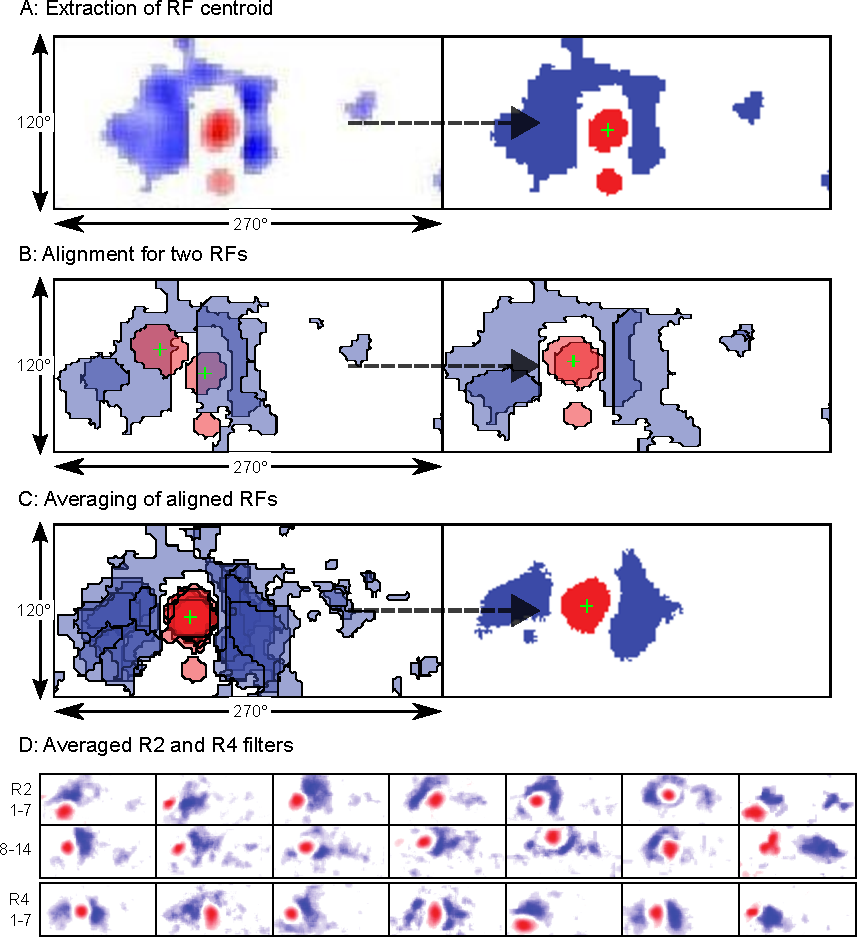
\includegraphics{figures/avkernels}
\caption{The algorithm for obtaining average RFs.}{
A: The raw image (left) is thresholded so as to give excitatory and inhibitory regions of uniform intensity (right).
The `centre' is then calculated as the centroid of the largest excitatory region (+).
B: Aligning two RFs.
The new centre is taken as the average of the centre of both RFs and the RFs are then shifted so that the centres are aligned.
C: Averaging the RFs for this glomerulus over all flies ($N=7$), following alignment.
Note that this the left-hemispheric version; the right-hemispheric version is its mirror.
Data are all for R4d glomerulus 1 neurons.}
\label{fig:avkernels}
\end{figure}


\subsection{Can we replicate behavioral experiments?}

\subsubsection{Population activity}
\include{tab_patterns}

\subsubsection{Could these neurons discriminate visual patterns?}

\subsubsection{Rotational image difference function}
Here we have used a modified version of the \ac{RIDF} \cite{Philippides2011,Zeil2003}.
$$
r(I,J,\bm{G},\theta) = \frac{1}{|\bm{G}|\cdot mn} {\sum\limits_{K \in \bm{G}} \sum\limits^n_{i=1} \sum\limits^m_{j=1} (I_{i,j}-J_{i,j})^2 \cdot {K_{i,j}}(\theta)^2}
$$

\begin{figure}
\centering
\includegraphics{figures/recap}
\caption{Simulation of fly pattern discrimination paradigm. A standard experimental paradigm for testing the pattern discrimination abilities of \emph{Drosophila} \protect\cite{Ernst1999} can be replicated in simulation.
A: A diagram showing Buridan's paradigm \protect\cite{Bulthoff1982,Gotz1980}. If a fly is placed in an arena between two large vertical bars, it will walk back and forth until exhaustion.
B and C: The mean output of R2 (blue) and R4d (green) filters, from different headings, to bars of different widths. The blue crosses in A indicate the points from which bars B and C are being viewed.
D: The fly is held tethered in a drum. As the fly attempts to rotate about its yaw-axis, the drum rotates in the opposite direction, thus allowing the fly to select the portion of the pattern in view.
By monitoring the fly's heading, one can surmise whether there is a spontaneous preference for one of the patterns.
Whether the fly can learn to head towards one pattern is tested by adding a laser that punishes the fly for facing one of the patterns.
Shown inside the drum are the visual \acp{RF} for one pair of left- and right-hemispheric glomeruli.
E and F: The \ac{rms} difference in output for R2 (blue) and R4d (green) neurons as the pattern is rotated.
The reference activities are the \ac{RF} outputs when the simulated flies are at 0\degree.
Patterns with a greater difference in activity at 0\degree\ \emph{vs} 90\degree\ should be more discriminable by flies.
For two pairs of patterns we show that there is a much smaller difference in output when the triangles are aligned about the vertical centre of mass (E) than not (F).
This mirrors real flies' performance on this task \protect\cite{Ernst1999}.}
\label{fig:recap}
\end{figure}


\subsection{What information is preserved in these neurons?}
Neural networks were used as a means of testing what properties of a visual stimulus can be encoded in a simple network.
The neural networks for this section were implemented using the \texttt{Netlab} toolbox for Matlab \cite{netlab}.
Two-layer feedforward networks with 10 hidden units, optimised with the scaled conjugate gradient function, were used throughout.

The stimuli with which the networks were trained were a series of black `blobs' on a white background.
The blobs were based on ellipses with a fixed ratio between the lengths of the major and minor axes, with the radii modified with complex waves:
$$
r \le \left(\frac{\cos^2 \theta}{2} + \frac{\sin^2 \theta}{a} \right)^{-1} + W(\theta)
$$
where $a$ is the length of the major axis and $W(\theta)$ is a complex wave defined as:
$$
W(\theta) = \sum_{i=1}^n W_i(\theta) = \sum_{i=1}^n A_i \sin f_i (\theta+\phi_i) 
$$
where $A_i$, $f_i$ and $\phi_i$ describe the maximum amplitude, frequency and phase shift of the wave $W_i(\theta)$, respectively.

\subsubsection{Can networks extract stimulus position?}


\bibliography{library}
\bibliographystyle{apacite}

\end{document}
